A mechanical doll is a doll which automatically repeats a specific sequence of motions.

In Japan, many mechanical dolls have been created since ancient times.
The motions of a mechanical doll are controlled by a \textbf{circuit} that consists of \textbf{devices}.
The devices are connected with tubes. Each device has one or two \textbf{exits}, and can have
arbitrarily many (possibly zero) \textbf{entrances}. Each tube connects an exit of a device to
an entrance of the same or another device. Exactly one tube is connected to each
entrance, and exactly one tube is connected to each exit.

To describe how the doll makes motions, consider a \textbf{ball} that is placed on one of the
devices. The ball travels through the circuit. At each step of the travel, the ball leaves
the device using one of its exits, travels along the tube connected to the exit and enters
the device at the other end of the tube.

There are three types of devices: \textbf{origin}, \textbf{trigger}, and \textbf{switch}. There are exactly one
origin, $M$ triggers, and $S$ switches ($S$ can be zero). You must decide the value of $S$.

Each device has a unique serial number.
The origin is the device where the ball is initially placed. It has one exit. Its serial
number is $0$.

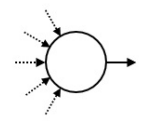
\includegraphics{1.png}


A trigger causes the doll to make a specific motion whenever the ball enters it. Every
trigger has one exit. The serial numbers of the triggers are from $1$ through $M$.

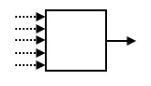
\includegraphics{2.png}

Each switch has two exits, which are called `X' and `Y'. The \textbf{state} of a switch is either
`X' or `Y'. After the ball enters a switch, it leaves the switch using the exit given by the
current state of the switch. After that, the switch changes its state to the opposite one.
Initially, the state of every switch is `X'. The serial numbers of the switches are from $-1$ through $-S$.

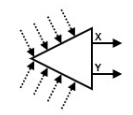
\includegraphics{3.png}

You are given the number of triggers $M$. You are also given a sequence $A$ of length $N$,
each of whose element is a serial number of a trigger. Each trigger might appear some
(possibly zero) times in the sequence $A$. Your task is to create a circuit that satisfies
the following conditions:

\begin{itemize}
    \item The ball returns to the origin after some steps.
    \item When the ball first returns to the origin, the state of every switch is `X'.
    \item The ball first returns to the origin after entering triggers exactly $N$ times. The
serial numbers of the triggers, in the order that they are entered, are $A_0,A_1,\ldots,A_{N-1}$.
    \item Let $P$ be the total number of state changes of all switches caused by the ball
before the ball first returns to the origin. The value of $P$ doesn't exceed $20\,000\,000$.
\end{itemize}

At the same time, you don't want to use too many switches.

\textbf{Implementation details}

You should implement the following procedure.

\begin{itemize}
    \item \texttt{create\_circuit(int M, int[] A)}
    \begin{itemize}
        \item $M$: the number of triggers.
        \item $A$: an array of length $N$, giving the serial numbers of the triggers the ball needs to enter, in the order they are to be entered. 
        \item This procedure is called exactly once. \item Note that the value of $N$ is the length of the array $A$, and can be obtained as indicated in the implementation notice.
    \end{itemize}
\end{itemize}
Your program should call the following procedure to answer.
\begin{itemize}
\item \texttt{answer(int[] C, int[] X, int[] Y)}
\begin{itemize}
    \item $C$: an array of length $M+1$. The exit of the device $i$ ($0 \le i \le M$) is connected to
the device $C[i]$.
    \item $X$, $Y$: arrays of the same length. The length $S$ of these arrays is the number of the
switches. For the switch $-j$ ($1 \le j \le S$), its exit `X' is connected to the device $X[j - 1]$ and its exit `Y' is connected to the device $Y[j - 1]$.
    \item Every element of $C$, $X$, and $Y$ must be an integer between $-S$ and $M$, inclusive.
    \item $S$ must be at most $400\,000$.
    \item This procedure must be called exactly once.
    \item The circuit represented by $C$, $X$, and $Y$ must satisfy the conditions in the problem
statement.
\end{itemize}
\end{itemize}


If some of the above conditions are not satisfied, your program is judged as \textbf{Wrong
Answer}. Otherwise, your program is judged as \textbf{Accepted} and your score is calculated
by $S$(see Subtasks).